\subsection{Descripción del problema.}

\vspace*{0.3cm}

Dado un \textbf{tablero de ajedrez de tamaño $n$x$n$ y $k$ caballos ocupando
inicialmente ciertos casilleros (aleatorios)} del mismo, el objetivo consiste
en \textbf{reunir a todos los caballos en un mismo casillero, minimizando la
cantidad total de movimientos realizados}. Esta cantidad equivale a
\textbf{la suma de los movimientos de todos los caballos} en el tablero.

Un caballo $k$ puede moverse únicamente \textbf{respetando los movimientos
válidos según las reglas del ajedrez}. Además, \textbf{un casillero puede
estar ocupado por más de un caballo simultáneamente}.

\vspace*{0.5cm}

\textbf{Ejemplo:}

En un tablero de 8x8, con 3 caballos en las posiciones [2,2], [5,5] y [2,8],
la menor cantidad de saltos posibles es 4, haciendo que los caballos de los
extremos cayan hacia la posición del caballo del medio[5,5], como se puede ver
en la siguiente imagen:

\begin{figure}[htb]
  \begin{center}
      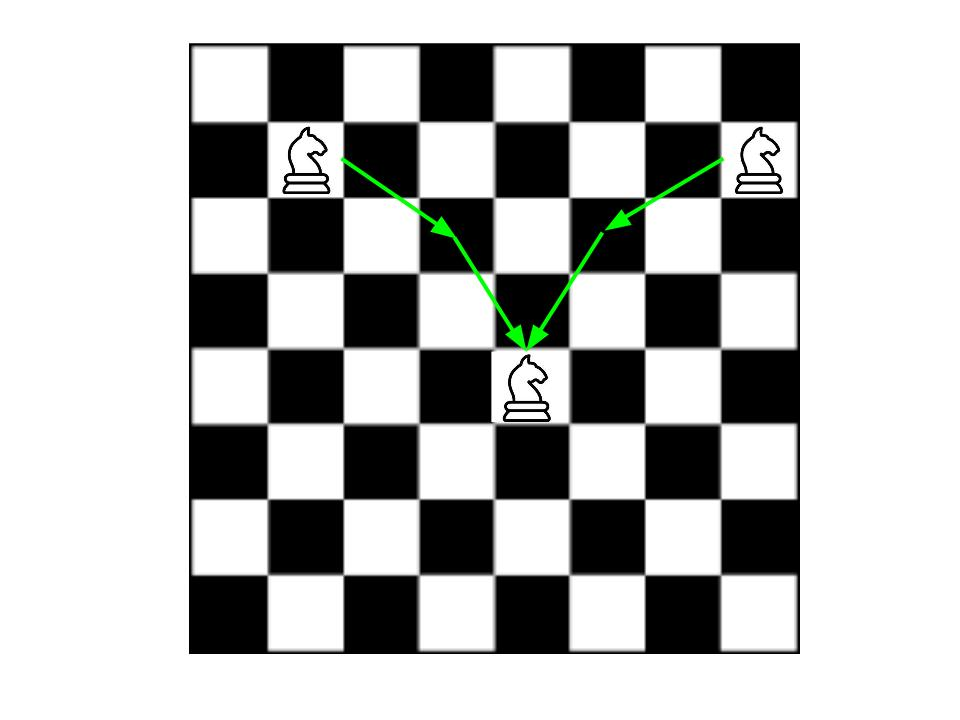
\includegraphics[scale=0.25]{imagenes/caballos.jpg}
  \end{center}
  \caption{ejemplo de tablero.}
\end{figure}


\newpage
\subsection{Desarrollo de la idea y pseudocódigo.}

\vspace*{0.3cm}


Para resolver este problema, utilizaremos $k$ tableros de $n$x$n$ casilleros,
uno por cada caballo. En cada tablero se calculará el costo para dicho caballo
de llegar a cada casillero, aplicando \textit{BFS} desde el casillero inicial,
quedando inválidos los casilleros que no pueden alcanzarse.

Luego se recorren todos los casilleros, sumando el valor de éstos en todos los
tableros (si son alcanzables), obteniendo así el costo de cada casillero para
cada caballo. De existir, el mínimo de estos valores será el casillero que
pueden alcanzar todos los caballos en la menor cantidad de saltos.

%\begin{codebox}
%\Procname{$\proc{puntoDeEncuentro}(caballos, n)$}
%\li $\id{tableros} \gets \emptyset$
%\li \For $caballo \in caballos$
%\li   \Do
%\li       $\proc{agregar}(\proc{crearTablero}(caballo,n), tableros)$
%      \End
%\li $\id{i} \gets 0$
%\li $\id{j} \gets 0$
%    $\id{min_i} \gets -1$
%    $\id{min_j} \gets -1$
%    $\id{min} \gets -1$
% \li \While $\id{i} < \id{n}$
% \li   \Do
% \li     \While $\id{j} < \id{n}$
% \li       \Do
% \li         $\id{sum} \gets 0$
% \li         $\id{caballo} \gets 0$
% \li         \While $\id{caballo} < \proc{tamaño}(caballos)$
% \li           \Do
%                 if (tableros[caballo][i][j] == -1)
%                   sum = -1
%                 else if (sum != -1)
%                   sum += tableros[caballo][i][j]
%                 end
%                 caballo++
%               \End
%             if (sum != -1 && (min == -1 || sum < min))
%               min = sum
%               min_i = i
%               min_j = j
%             end
%             j++
%         \End
%         i++
%       \End
%     if min == -1
%       \Return 'no'
%     else
% \li \Return min min_i min_j
% \end{codebox}
%
%
% crearTablero



\newpage
\subsection{Justificación de la resolución y demostración de correctitud.}

\vspace*{0.3cm}

La solución es el mínimo número de movimientos entre todos los caballos que
los deja en el mismo casillero.

Primero completamos cuanto le cuesta a cada caballo llegar a cada
casillero, para calcular esto tomamos al tablero como un grafo, cada
casillero como un nodo y los ejes los posibles saltos de caballo. Empezando
desde la posición del caballo, se recorre de una forma Breadth-First,
logrando de esta manera poner la cantidad mínima de saltos para cada
casillero alcanzable, ya que el algoritmo BFS obtiene todos los caminos
mínimos desde un nodo inicial.

Luego, simplemente es cuestión de obtener el mínimo de la sumatoria para cada casillero.
Recorremos todos los casilleros para cada tablero (de cada caballo),
tomando el valor mínimo (únicamente si es posible llegar a ese casillero
con todos los caballos).
Este mínimo (si existe) es una solución óptima.

\newpage
\subsection{Análisis de complejidad.}

\vspace*{0.3cm}

\textcolor{red}{\textbf{completar!}}



\newpage
\subsection{Experimentación y gráficos.}

\vspace*{0.3cm}

\subsubsection{Test 1 - benchmark caso aleatorio}

\textcolor{red}{\textbf{completar!}}


\newpage
\subsubsection{Test 2 - benchmark del peor caso}

Este ejercicio no tiene mejor y peor caso, todos tardan lo mismo.
Porque en todos los casos se generan los tableros para todos los caballos
y también se busca el mínimo en todos los casilleros.-
\textcolor{red}{\textbf{completar!}}


\newpage
\subsubsection{Test 3 - benchmark del mejor caso}

\textcolor{red}{\textbf{completar!}}
